\chapter{Results}

\section{Sampling Inacurracies}
The faces in the set of given scans all contain large holes around the ears and the eyes. In effect, the projected sample points are often off target, because due to this circumstance the mesh vertex with the most similar direction is likely farther away at a suboptimal location. This leads to the projected line being distortet.
\begin{figure}[h!]
    \includegraphics[width=.7\textwidth]{./resources/img/linefeatures_eyes.pdf}
    \caption{Line Features}
    \label{fig:linefeature_comparison}
\end{figure}
\viscomment{find dataset with stronger disparity}

On different data sets the performance of the projection of the line features for a large number of
samples, i.e. 30, varied significantly. Overall, one can say that the distortion of a projected line increases with the amount of sample points if the scan contains large holes.
An easy workaround was to reduce the number/amount of sample points. By using only 5-10 sample points per curve some datasets rendered near perfect results on a ``control dataset''. However, when the holes are too large this workaround also fails. This circumstance leaves room for discussion. As long as the method is dependent on the data from the scans - the size of the holes in the meshs - it lacks generality and generality is exactly the basis for feasible and reproducable registration results.\\

\section{The effect of Line Features}
In this section we will exhibit/illustrate the effect the incorporation of line features has on the registration results. We use up-close images on the various feature regions of different fits with and without line features and compare them to one another and the targets.
\begin{figure}[h!]
    \includegraphics[width=\textwidth]{./resources/img/00029_eyes_comparison.pdf}
\caption{Eyes}
\label{fig:fiteyes}
% reference in text by \ref{$figure-name}
\end{figure}

\begin{figure}[h!]
    \includegraphics[width=\textwidth]{./resources/img/00029_left_ear_comparison.pdf}
\caption{Ears}
\label{fig:fitears}
% reference in text by \ref{$figure-name}
\end{figure}

\begin{figure}[h!]
    \centering
    \includegraphics[width=.6\textwidth]{./resources/img/00029_mouth_comparison.pdf}
    \label{fig:00029_mouth_comparison}
    \caption{From top to bottom: fit without line features, fit with line features, target with mean texture projection}
\end{figure}

\section{Registration quality}

\subsection{Visualized Distance}
with line features
\begin{figure}[h]
    \centering
    \subfloat[target front]{\includegraphics[width=.8\textwidth]{./resources/img/00029_textured_target.pdf}}\\
    \subfloat[deformed mean]{
\includegraphics[width=.8\textwidth]{./resources/img/00029_fit.pdf}}\\
    \subfloat[distance]{\includegraphics[width=.8\textwidth]{./resources/img/00029_distmap.pdf}}
    \caption{}
\label{fig:distmap}
% reference in text by \ref{$figure-name}
\end{figure}

\begin{figure}[h!]
    \subfloat[target front]{}
    \subfloat[deformed mean]{}
    \subfloat[distance]{}

    \subfloat[target left]{}
    \subfloat[deformed mean]{}
    \subfloat[distance]{}

    \subfloat[target right]{}
    \subfloat[deformed mean]{}
    \subfloat[distance]{}
    \caption{}
\label{fig:distmap}
% reference in text by \ref{$figure-name}
\end{figure}

\begin{figure}[h!]
    \subfloat[target]{}
    \subfloat[deformed mean]{}
    \subfloat[distance]{}
    \caption{}
\label{fig:distmap}
% reference in text by \ref{$figure-name}
\end{figure}

\subsection{Caricatures}
Maximum scaling two times. Prominent features, become more prominent, but of course artifacts also become more prominent
Caricatures rendered by adding scaled displacement fields

\begin{figure}[h!]
    \centering
    \subfloat[130\% scale]{\includegraphics[width=.8\textwidth]{./resources/img/00029_caricature_1_3.pdf}}\\
    \subfloat[160\% scale]{\includegraphics[width=.8\textwidth]{./resources/img/00029_caricature_1_6.pdf}}\\
    \subfloat[200\% scale]{\includegraphics[width=.8\textwidth]{./resources/img/00029_caricature_2.pdf}}\\
    \subfloat[130\% scale]{\includegraphics[width=.8\textwidth]{./resources/img/00303_caricature_1_3.pdf}}\\
    \subfloat[160\% scale]{\includegraphics[width=.8\textwidth]{./resources/img/00303_caricature_1_6.pdf}}\\
    \subfloat[200\% scale]{\includegraphics[width=.8\textwidth]{./resources/img/00303_caricature_2.pdf}}
   \caption{}
\label{fig:caricature}
% reference in text by \ref{$figure-name}
\end{figure}

\subsection{Effects of the Covariance Function}
A Gaussian Kernel
00125 - scan of old man --> wrinkles can't be modelled through this smooth definition of covariance - adjust covariance function
\section{Discussion \& Future Work}
